\caulc
\begin{ex}%[1D2N2-4]%[TDMZZ23]%[ Nguyễn Sơn Thành, Trần Văn Thiện]
	Cho cấp số cộng $(u_n)$ có $u_2 = 1$ và $u_1 = 3$. Giá trị của $u_3$ bằng
	\choice
	{\True $-1$}
	{$4$}
	{$5$}
	{$7$}
	\loigiai{
		Ta có công sai $d$ của cấp số cộng được tính bằng công thức
		$d = u_2 - u_1 = 1 - 3 = -2$.\\
		Giá trị của số hạng $u_3$ là
		$u_3 = u_2 + d = 1 + (-2) = -1$.
	}
\end{ex}

\begin{ex}%[1D6H4-3]%[TDMZZ23]%[ Nguyễn Sơn Thành, Trần Văn Thiện]
	Tập nghiệm của bất phương trình $\ln\left(x^3 - 3x^2 + 6x\right) > \ln\left(x^3 - 2x^2\right)$ là
	\choice
	{$(0; 6)$}
	{\True $(2; 6)$}
	{$(-\infty; 0)$}
	{$(6; +\infty)$}
	\loigiai{
		Điều kiện xác định:
		$\heva{&x^3 - 3x^2 + 6x > 0 \\ &x^3 - 2x^2 > 0} \Leftrightarrow \heva{&x\left(x^2 - 3x + 6\right) > 0 \\ &x^2(x - 2) > 0} \Leftrightarrow \heva{&x > 0 \\ &x > 2} \Leftrightarrow x > 2$.\\
		Với điều kiện $x > 2$, bất phương trình đã cho tương đương với
		\begin{eqnarray*}
			& & x^3 - 3x^2 + 6x > x^3 - 2x^2 \\
			&\Leftrightarrow & x^2 - 6x < 0 \\
			&\Leftrightarrow & 0 < x < 6.
		\end{eqnarray*}
		Kết hợp với điều kiện $x > 2$, ta được $2 < x < 6$.\\
		Vậy tập nghiệm của bất phương trình là $(2; 6)$.
	}
\end{ex}

\begin{ex}%[1H8H5-4]%[TDMZZ23]%[ Nguyễn Sơn Thành, Trần Văn Thiện]
	Cho hình lập phương $ABCD. A'B'C'D'$ có cạnh bằng $a$. Hãy tính $\mathrm{d}(A'B,C'D)$.
	\choice
	{\True $a$}
	{$a\sqrt{2}$}
	{$a\sqrt{3}$}
	{$\dfrac{a\sqrt{2}}{2}$}
	\loigiai{
		\immini{Ta có $A'B \subset (ABB'A')$ và $C'D \subset (DCC'D')$.\\
			Lại có mặt phẳng $(ABB'A') \parallel (DCC'D')$ nên khoảng cách giữa hai đường thẳng chéo nhau $A'B$ và $C'D$ chính là khoảng cách giữa hai mặt phẳng song song chứa chúng.\\
			Suy ra $\mathrm{d}(A'B,C'D) = \mathrm{d}\left((ABB'A'), (DCC'D')\right)$.\\
			Mặt khác, vì $ABCD. A'B'C'D'$ là hình lập phương nên $AD \perp (ABB'A')$ tại $A$ và $AD \perp (DCC'D')$ tại $D$.\\
			Do đó $\mathrm{d}\left((ABB'A'), (DCC'D')\right) = AD = a$.\\
			Vậy $\mathrm{d}(A'B,C'D) = a$.}{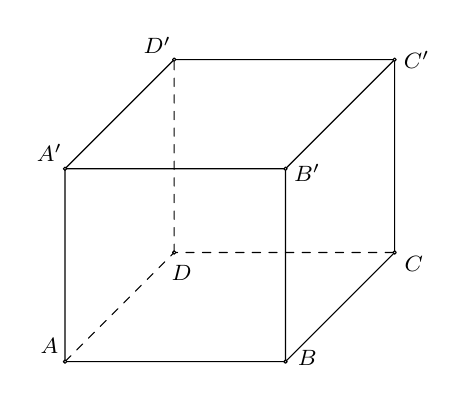
\begin{tikzpicture}[scale=0.7, font=\footnotesize,line join=round, line cap=round, >=stealth]
				\path
				(0:0) coordinate (D)
				(0:4) coordinate (C)
				(-135:2.8) coordinate (A)
				+(C) coordinate (B)
				\foreach \x in {A,B,C,D}{(\x)+(90:3.5) coordinate (\x')}
				;
				\draw[dashed] (A)--(D)--(C) (D)--(D');
				\draw 
				(A)--(B)--(B')--(A')--cycle
				(B)--(C)--(C')--(B')  (A')--(D')--(C')
				;
				\foreach \x/\g in {A/135,B/10,C/-30,D/-70,A'/135,B'/-10,C'/0,D'/140}\draw[fill=white] (\x) circle (.03) +(\g:.4) node{$\x$};
		\end{tikzpicture}}
	}
\end{ex}

\begin{ex}%[1D6H4-4]%[TDMZZ23]%[ Nguyễn Sơn Thành, Trần Văn Thiện]
	Nghiệm của phương trình $3^{x+2}=1$ là
	\choice
	{$x=0$}
	{$x=-1$}
	{$x=2$}
	{\True $x=-2$}
	\loigiai{
		Ta có $3^{x+2}=1 \Leftrightarrow 3^{x+2}=3^0 \Leftrightarrow x+2=0 \Leftrightarrow x=-2$.\\
		Vậy nghiệm của phương trình là $x=-2$.
	}
\end{ex}

\begin{ex}%[2H5N1-2]%[TDMZZ23]%[ Nguyễn Sơn Thành, Trần Văn Thiện]
	Trong không gian $Oxyz$, một vectơ pháp tuyến của mặt phẳng $(P)\colon 3x - z + 4 = 0$ tương ứng là
	\choice
	{$\overrightarrow{n}_1=(3;0;4)$}
	{$\overrightarrow{n}_2=(3;-1;4)$}
	{\True $\overrightarrow{n}_3=(3;0;-1)$}
	{$\overrightarrow{n}_4=(3;0;-4)$}
	\loigiai{
		Phương trình mặt phẳng $(P)\colon 3x - z + 4 = 0$ có thể viết lại là $(P)\colon3x + 0y - 1z + 4 = 0$.\\
		Suy ra mặt phẳng $(P)$ có một vectơ pháp tuyến là $\overrightarrow{n} = (3;0;-1)$.
	}
\end{ex}

\begin{ex}%[2D1H3-2]%[TDMZZ23]%[ Nguyễn Sơn Thành, Trần Văn Thiện]
	Cho bảng biến thiên của hàm số $f(x)$ như hình vẽ bên dưới. Giá trị lớn nhất của hàm số $y=f(x)$ trên khoảng $(-\infty;0)$ là
	\begin{center}
		
\begin{tikzpicture}
			\tkzTabInit[nocadre=false,lgt=1.2,espcl=2.5,deltacl=0.67]
			{$x$ /0.6,$f'(x)$ /0.6,$f(x)$ /2}
			{$-\infty$,$-1$,$3$,$+\infty$}
			\tkzTabLine{,+,0,-,0,+,}
			\tkzTabVar{-/ $-\infty$ , +/ $5$ , -/ $-2$ , +/ $+\infty$}
		\end{tikzpicture}
	\end{center}
	\choice
	{$-1$}
	{\True $5$}
	{$+\infty$}
	{$3$}
	\loigiai{
		Dựa vào bảng biến thiên, ta xét hàm số $y=f(x)$ trên khoảng $(-\infty;0)$:\\
		Hàm số đồng biến trên khoảng $(-\infty;-1)$ và nghịch biến trên khoảng $(-1;0)$.\\
		Do đó, hàm số đạt cực đại tại $x=-1$ và giá trị cực đại là $f(-1)=5$.\\
		Đồng thời, đây cũng là giá trị lớn nhất của hàm số trên khoảng $(-\infty;0)$.\\
		Vậy $\max\limits_{(-\infty;0)} f(x) = 5$.
	}
\end{ex}

\begin{ex}%[2D4N1-3]%[TDMZZ23]%[ Nguyễn Sơn Thành, Trần Văn Thiện]
	Họ nguyên hàm của hàm số $f(x)=4x^3-\dfrac{1}{\sin^2 x}$ là
	\choice
	{\True $F(x)=x^4+\cot x+C$}
	{$F(x)=x^4-\cot x+C$}
	{$F(x)=x^4+\dfrac{1}{\cos^2 x}x+C$}
	{$F(x)=x^4-\dfrac{1}{\cos^2 x}x+C$}
	\loigiai{
		Ta có $\displaystyle\int f(x)\mathrm{\,d}x = \displaystyle\int \left(4x^3-\dfrac{1}{\sin^2 x}\right)\mathrm{\,d}x = x^4 - (-\cot x) + C = x^4+\cot x+C$.
	}
\end{ex}

\begin{ex}%[2H2H1-2]%[TDMZZ23]%[ Nguyễn Sơn Thành, Trần Văn Thiện]
	Cho hình lăng trụ đứng $ABC. A'B'C'$. Hỏi khi đó $\overrightarrow{AC} + \overrightarrow{B'B} + \overrightarrow{CB}$ bằng với véctơ nào dưới đây?
	\choice
	{$\overrightarrow{0}$}
	{$\overrightarrow{BC}$}
	{ $\overrightarrow{AB'}$}
	{\True $\overrightarrow{A'B}$}
	\loigiai{
		\immini{Ta có $\overrightarrow{AC} + \overrightarrow{B'B} + \overrightarrow{CB} = \left(\overrightarrow{AC} + \overrightarrow{CB}\right) + \overrightarrow{B'B} = \overrightarrow{AB} + \overrightarrow{B'B}$.\\
			Vì $ABC. A'B'C'$ là hình lăng trụ nên các cạnh bên song song và bằng nhau, suy ra $\overrightarrow{B'B} = \overrightarrow{A'A}$.\\
			Do đó, ta có $ \overrightarrow{AB} + \overrightarrow{B'B} = \overrightarrow{A'A} + \overrightarrow{AB} = \overrightarrow{A'B}$.\\
			Vậy tổng các véctơ đã cho bằng $\overrightarrow{A'B}$.}{	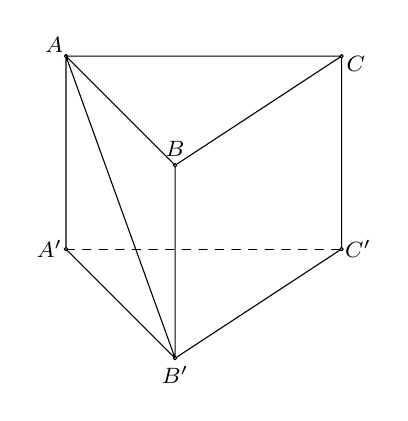
\begin{tikzpicture}[scale=0.7, font=\footnotesize,line join=round, line cap=round, >=stealth]
				\path
				(0:0) coordinate (A)
				(0:5) coordinate (C)
				(-45:2.8) coordinate (B)
				\foreach \x in {A,B,C}{(\x)+(-90:3.5) coordinate (\x')}
				;
				\draw[dashed] (A')--(C') ;
				\draw 
				(A)--(B)--(C)--cycle
				(A)--(A')--(B')--(B) (C)--(C')--(B') (A)--(B') 
				;
				\foreach \x/\g in {A/135,B/90,C/-30,A'/180,B'/-90,C'/0}\draw[fill=white] (\x) circle (.03) +(\g:.3) node{$\x$};
		\end{tikzpicture}}
		
	}
\end{ex}

\begin{ex}%[2D1H5-7]%[TDMZZ23]%[ Nguyễn Sơn Thành, Trần Văn Thiện]
	Đồ thị của hàm số $y = \dfrac{x^2 - 5x + 7}{x - 2}$ có tâm đối xứng là
	\choice
	{\True $(2;-1)$}
	{$(2;-3)$}
	{$(3;2)$}
	{$(2;1)$}
	\loigiai{
		Tập xác định $\mathscr{D} = \mathbb{R} \setminus \{2\}$.\\
		Ta có $y = \dfrac{x^2 - 5x + 7}{x - 2} = x - 3 + \dfrac{1}{x - 2}$.\\
		Đồ thị hàm số có đường tiệm cận đứng là $x = 2$ và đường tiệm cận xiên là $y = x - 3$.\\
		Đồ thị hàm số nhận giao điểm hai đường tiệm cận làm tâm đối xứng.\\
		Tọa độ tâm đối xứng là nghiệm của hệ phương trình
		$\heva{&x=2\\&y=x-3} \Leftrightarrow \heva{&x=2\\&y=-1.}$\\
		Vậy đồ thị hàm số có tâm đối xứng là $(2; -1)$.
	}
\end{ex}

\begin{ex}%[2D3N1-2]%[TDMZZ23]%[ Nguyễn Sơn Thành, Trần Văn Thiện]
	Cho hai mẫu số liệu ghép nhóm $M_1$, $M_2$ với bảng tần số ghép nhóm như sau:
	\begin{center}
		\begin{tabular}{cl}
			\textit{Nhóm $M_1$} &
			\begin{tabular}{|c|c|c|c|c|c|c|}
				\hline
				Nhóm & $[2;3)$ & $[3;4)$ & $[4;5)$ & $[5;6)$ & $[6;7)$ & $[7;8)$ \\
				\hline
				Tần số & $5$ & $11$ & $6$ & $4$ & $6$ & $5$ \\
				\hline
			\end{tabular}
		\end{tabular}
		
		\vspace{5pt}
		\begin{tabular}{cl}
			\textit{Nhóm $M_2$} &
			\begin{tabular}{|c|c|c|c|c|c|c|}
				\hline
				Nhóm & $[4;6)$ & $[6;8)$ & $[8;10)$ & $[10;12)$ & $[12;14)$ & $[14;16)$ \\
				\hline
				Tần số & $8$ & $3$ & $6$ & $4$ & $6$ & $5$ \\
				\hline
			\end{tabular}
		\end{tabular}
	\end{center}
	Hãy so sánh khoảng biến thiên $a$, $b$ tương ứng của hai mẫu số liệu $M_1$, $M_2$?
	\choice
	{$a=b$}
	{$a>b$}
	{$b=3a$}
	{\True $b=2a$}
	\loigiai{
		Khoảng biến thiên của mẫu số liệu ghép nhóm là hiệu số giữa đầu mút phải của nhóm cuối cùng và đầu mút trái của nhóm đầu tiên.
		\begin{itemize}
			\item Đối với mẫu số liệu $M_1$: Khoảng biến thiên là $a = 8 - 2 = 6$.
			\item Đối với mẫu số liệu $M_2$: Khoảng biến thiên là $b = 16 - 4 = 12$.
		\end{itemize}
		Ta thấy $12 = 2 \cdot 6$, suy ra $b = 2a$.
	}
\end{ex}

\begin{ex}%[2H2N2-2]%[TDMZZ23]%[ Nguyễn Sơn Thành, Trần Văn Thiện]
	Trong không gian $Oxyz$, cho điểm $A(2;3;-1)$. Tọa độ của điểm đối xứng với $A$ qua mặt phẳng $(Oxz)$ là
	\choice
	{$(2;3;-1)$}
	{\True $(2;-3;-1)$}
	{$(-2;-3;1)$}
	{$(-2;3;1)$}
	\loigiai{
		Tọa độ điểm đối xứng với điểm $M(x;y;z)$ qua mặt phẳng $(Oxz)$ là $M'(x;-y;z)$.\\
		Áp dụng công thức trên, điểm đối xứng với điểm $A(2;3;-1)$ qua mặt phẳng $(Oxz)$ có tọa độ là $(2;-3;-1)$.
	}
\end{ex}

\begin{ex}%[2D4H3-2]%[TDMZZ23]%[ Nguyễn Sơn Thành, Trần Văn Thiện]
	Cho hình phẳng $(H)$ giới hạn bởi các đường $y=x^3-2x^2-x$, $y=x^2-3x$. Diện tích hình phẳng $(H)$ bằng
	\choice
	{\True $\dfrac{1}{2}$}
	{$1$}
	{$\dfrac{1}{2}\pi$}
	{$2$}
	\loigiai{
		\immini{Phương trình hoành độ giao điểm của hai đường là
			$$x^3-2x^2-x=x^2-3x \Leftrightarrow x^3-3x^2+2x=0 \Leftrightarrow \hoac{&x=0\\&x=1\\&x=2.}$$}{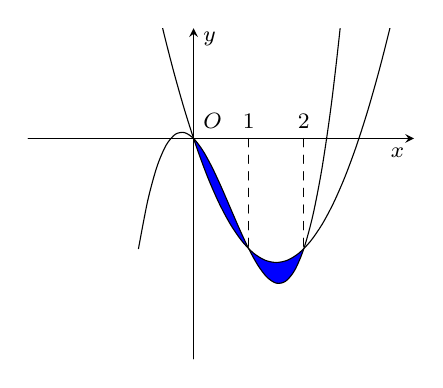
\begin{tikzpicture}[scale=0.7, font=\footnotesize,line join=round, line cap=round, >=stealth]
				
				\def \a{0}
				\def \b{2}
				\def\f(#1){(#1)^2-3*(#1)}
				\def\g(#1){(#1)^3-2*(#1)^2-(#1)}
				
				\fill[blue,smooth]
				plot[domain=\a:\b] (\x,{\f(\x)})
				-- plot[domain=\b:\a] (\x,{\g(\x)})
				-- cycle;
				
				\draw[->] (-3,0) -- (4,0);
				\draw[->] (0,-4) -- (0,2); 
				\clip(-3,-4) rectangle (4,2); 
				\draw[dashed] (1,0) -- (1,-2);
				\draw[dashed] (2,0) -- (2,-2);
				\draw[smooth,black]	plot[domain=-1:4]	(\x,{\f(\x)});
				\draw[smooth,black]	plot[domain=-1:3]	(\x,{\g(\x)});
				\node at (1,0) [above] {$1$};
				\node at (2,0)  [above] {$2$};
				
				\node at (3.7,0) [below] {$x$};
				\node at (0,1.8) [right] {$y$};
				\node at (0,0) [above right] {$O$};
		\end{tikzpicture}		}
		Diện tích hình phẳng $(H)$ cần tìm là
		\begin{eqnarray*}
			S &=& \displaystyle\int\limits_0^2 \left|x^3-3x^2+2x\right| \mathrm{\,d}x \\
			&=& \displaystyle\int\limits_0^1 \left|x^3-3x^2+2x\right| \mathrm{\,d}x + \displaystyle\int\limits_1^2 \left|x^3-3x^2+2x\right| \mathrm{\,d}x \\
			&=& \displaystyle\int\limits_0^1 \left(x^3-3x^2+2x\right) \mathrm{\,d}x - \displaystyle\int\limits_1^2 \left(x^3-3x^2+2x\right) \mathrm{\,d}x \\
			&=& \left.\left(\dfrac{x^4}{4}-x^3+x^2\right)\right|_0^1 - \left.\left(\dfrac{x^4}{4}-x^3+x^2\right)\right|_1^2 \\
			&=& \dfrac{1}{4} - \left(0-\dfrac{1}{4}\right) \\
			&=& \dfrac{1}{2}.
		\end{eqnarray*}
	}
\end{ex}
\cauds
\begin{ex}%[2H5H2-6]%[Dương Công Tạo]
	Trong không gian $Oxyz$, cho đường thẳng $d\colon \dfrac{x}{1}=\dfrac{y-1}{2}=\dfrac{z-2}{2}$ và điểm $A(4;5;5)$. Biết rằng $M$ là điểm chạy trên đường thẳng $d$.
	\choiceTF
	{\True Một vectơ chỉ phương của $d$ là $\overrightarrow{u} = (1;2;2)$}
	{Hình chiếu vuông góc của điểm $A$ trên $d$ là $H(2;1;4)$}
	{\True $\mathrm{d}\left(A,d\right)= \sqrt{5}$}
	{Biết rằng $\triangle OAM$ vuông tại $O$. Khi đó tung độ của điểm $M$ bằng $\dfrac{5}{4}$}
	\loigiai{
		\begin{itemchoice}
			\itemch Một vectơ chỉ phương của $d$ là $\overrightarrow{u} = (1;2;2)$.
			\itemch Phương trình tham số của $d\colon \heva{&x=t\\&y=1+2t\\&z=2+2t},(t\in\mathbb{R})$.\\
			Gọi $H$ là hình chiếu của điểm $A(4;5;5)$ lên $d$ thì $H(t;1+2t;2+2t)$.\\
			Ta có $\overrightarrow{AH}=(t-4;2t-4;2t-3)$, vectơ chỉ phương của $d$ là $\overrightarrow{u} = (1;2;2)$.\\
			Vì $H$ là hình chiếu của điểm $A$ lên $d$ nên $\overrightarrow{u}\cdot\overrightarrow{AH}=0\Leftrightarrow1\cdot (t-4)+2\cdot(2t-4)+2\cdot(2t-3)=0\Leftrightarrow t=2$.\\
			Với $t=2$ suy ra $H(2;5;6)$.
			\itemch Khoảng cách từ điểm $A$ đến đường thẳng $d$ là \[\mathrm{d}\left(A,d\right)=AH=\sqrt{(2-4)^2+(5-5)^2+(6-5)^2}=\sqrt{5}.\]
			\itemch Gọi $M(x;y;z)$ là điểm cần tìm.\\
			Ta có $\triangle OAM$ vuông tại $O$ suy ra $\overrightarrow{OA}\cdot\overrightarrow{OM}=0$.\quad(*)\\
			Mà $\overrightarrow{OA}=(4;5;5)$, $\overrightarrow{OM}=(x;y;z)$.\\
			Do đó, $(*)\Leftrightarrow 4x+5y+5z=0$.\quad(1)\\
			Mặt khác $M\in d\Rightarrow M(t;1+2t;2+2t)$.\quad(2)\\
			Thế (1) vào (2) ta được $4t+5(1+2t)+5(2+2t)=0\Leftrightarrow24t+15=0\Leftrightarrow t=-\dfrac{5}{8}$.\\
			Vậy, tung độ của điểm $M$ là $1+2\cdot\left(-\dfrac{5}{8}\right)=-\dfrac{1}{4}$.
		\end{itemchoice}
	}
\end{ex}

\begin{ex}%[TDMZZ23]%[Hà Văn Hảo]%[2D4V3-1]
	Trong mặt phẳng tọa độ $Oxy$, cho hàm số $y=f(x)$ có đồ thị $(C)$. Biết rằng tâm đối xứng của $(C)$ là $I(0;2)$ và có $f'(x)=-\dfrac{3}{x^2}$.
	\choiceTF
	{\True $(C)$ có tiệm cận đứng là $x=0$}
	{\True $f(x)=\dfrac{2x+3}{x}$}
	{\True Hai trục đối xứng của $(C)$ lần lượt là $y=x+2$, $y=-x+2$}
	{Diện tích phần hình phẳng giới hạn bởi $(C)$ và một trục đối xứng với đường thẳng $y=3$ là $0{,}96$ (\textit{làm tròn kết quả đến hàng phần trăm})}
	\loigiai{
		\begin{itemchoice}
			\itemch Ta có $f'(x) = -\dfrac{3}{x^2}$. Nguyên hàm của $f'(x)$ là $f(x) = \displaystyle\int \left(-\dfrac{3}{x^2}\right) \,\mathrm{d}x = \dfrac{3}{x} + C$.\\
			Vì đồ thị $(C)$ nhận $I(0;2)$ làm tâm đối xứng nên đường thẳng $x=0$ là tiệm cận đứng và đường thẳng $y=2$ là tiệm cận ngang.
			\itemch Từ tiệm cận ngang $y=2$, ta có $\displaystyle\lim_{x \to \pm\infty} f(x) = 2 \Rightarrow \displaystyle\lim_{x \to \pm\infty} \left(\dfrac{3}{x} + C\right) = 2 \Rightarrow C = 2$.\\
			Vậy hàm số là $f(x) = \dfrac{3}{x} + 2 = \dfrac{2x+3}{x}$.
			\itemch Đồ thị của hàm số phân thức hữu tỷ bậc nhất trên bậc nhất $y = \dfrac{ax+b}{cx+d}$ có hai trục đối xứng là các đường thẳng đi qua tâm đối xứng $I(x_0; y_0)$ và có hệ số góc $k = \pm 1$.\\
			Với $I(0;2)$, phương trình hai trục đối xứng là
			\[\hoac{&y - 2 = 1(x - 0) \\ &y - 2 = -1(x - 0)} \Leftrightarrow \hoac{&y = x + 2 \\ &y = -x + 2.}\]
			\itemch Trục đối xứng được chọn phải cắt cả đồ thị $(C)$ và đường thẳng $y = 3$ để tạo thành hình phẳng khép kín.\\
			Xét trục đối xứng $d\colon y = x+2$.\\
			Giao điểm của $(C)$ và $y = x+2$ là nghiệm của phương trình
			\[\dfrac{2x+3}{x} = x+2 \Leftrightarrow 2x+3 = x^2 + 2x \Leftrightarrow x^2 = 3 \Leftrightarrow x = \pm\sqrt{3}.\]
			Giao điểm của $(C)$ và $y = 3$ là nghiệm của phương trình
			\[\dfrac{2x+3}{x} = 3 \Leftrightarrow 2x+3 = 3x \Leftrightarrow x = 3.\]
			Giao điểm của $y=3$ và $y=x+2$ là $x=1$. \\
			Phần hình phẳng được giới hạn bởi các đường nằm trong khoảng giữa các giao điểm tương ứng (xét nhánh đồ thị dương $x > 0$ chứa các điểm $x = 1$, $x = \sqrt{3}$ và $x = 3$).\\
			Diện tích cần tìm là
			\allowdisplaybreaks
			\begin{eqnarray*}
				S &=& \displaystyle\int\limits_1^{\sqrt{3}} \left|(x+2)-3\right| \,\mathrm{d}x + \displaystyle\int\limits_{\sqrt{3}}^3 \left| \frac{2x+3}{x} - 3 \right| \,\mathrm{d}x\\
				&=& \displaystyle\int\limits_1^{\sqrt{3}} \left|x-1\right|\,\mathrm{d}x + \displaystyle\int\limits_{\sqrt{3}}^3 \left| \frac{3}{x} - 1 \right| \,\mathrm{d}x\\
				&\approx& 0{,}65.
			\end{eqnarray*}
		\end{itemchoice}
	}
\end{ex}

\begin{ex}%[2D6V2-4]%[TDMZZ23]%[Vũ Hồng Toàn]
	Người ta thiết kế một con súc sắc cân đối đồng chất có dạng đa diện $12$ mặt đều, trên đó có ba mặt $3$ chấm, bốn mặt $4$ chấm và năm mặt $5$ chấm. Tiến hành gieo ngẫu nhiên con súc sắc này hai lần liên tiếp. Gọi $A$ là biến cố lần thứ nhất xuất hiện mặt $3$ chấm, $B$ là biến cố tổng số chấm ở hai lần gieo bằng $7$.
	\choiceTF
	{\True $\mathrm{P}(A)=\dfrac{1}{4}$}
	{\True $\mathrm{P}(B\mid A)=\dfrac{1}{3}$}
	{\True $\mathrm{P}(B)=\dfrac{1}{6}$}
	{\True $\mathrm{P}(A\mid B)=\dfrac{1}{2}$}
	\loigiai{
		Con súc sắc có $12$ mặt cân đối đồng chất gồm: $3$ mặt $3$ chấm, $4$ mặt $4$ chấm và $5$ mặt $5$ chấm.\\
		Xác suất xuất hiện các mặt trong mỗi lần gieo là
		\begin{itemize}
			\item Xác suất xuất hiện mặt $3$ chấm là $\mathrm{P}(3) = \dfrac{3}{12} = \dfrac{1}{4}$.
			\item Xác suất xuất hiện mặt $4$ chấm là $\mathrm{P}(4) = \dfrac{4}{12} = \dfrac{1}{3}$.
			\item Xác suất xuất hiện mặt $5$ chấm là $\mathrm{P}(5) = \dfrac{5}{12}$.
		\end{itemize}
		\begin{itemchoice}
			\itemch Ta có $\mathrm{P}(A) = \mathrm{P}(3) = \dfrac{1}{4}$.
			\itemch Khi lần thứ nhất đã xuất hiện mặt $3$ chấm, để tổng số chấm bằng $7$ thì lần thứ hai bắt buộc phải xuất hiện mặt $4$ chấm.\\
			Xác suất để lần thứ hai xuất hiện mặt $4$ chấm là $\mathrm{P}(4) = \dfrac{1}{3}$.\\
			Do đó, $\mathrm{P}(B\mid A) = \dfrac{1}{3}$.
			\itemch Vì con súc sắc chỉ có các mặt $3$, $4$, $5$ chấm nên tổng số chấm bằng $7$ chỉ xảy ra trong hai trường hợp sau:
			\begin{enumerate}[{\bf TH 1.}]
				\item Lần một gieo được $3$ chấm, lần hai gieo được $4$ chấm.\\ Xác suất là
				$\mathrm{P}(3; 4) = \mathrm{P}(3) \cdot \mathrm{P}(4) = \dfrac{1}{4} \cdot \dfrac{1}{3} = \dfrac{1}{12}$.
				\item Lần một gieo được $4$ chấm, lần hai gieo được $3$ chấm.\\ Xác suất là
				$\mathrm{P}(4; 3) = \mathrm{P}(4) \cdot \mathrm{P}(3) = \dfrac{1}{3} \cdot \dfrac{1}{4} = \dfrac{1}{12}$.
			\end{enumerate}
			Xác suất của biến cố $B$ là
			\[\mathrm{P}(B) = \mathrm{P}(3; 4) + \mathrm{P}(4; 3) = \dfrac{1}{12} + \dfrac{1}{12} = \dfrac{1}{6}.\]
			\itemch Xác suất của biến cố $A \cap B$ là
			$\mathrm{P}(A \cap B) = \mathrm{P}(3; 4) = \dfrac{1}{12}$.\\
			Áp dụng công thức xác suất có điều kiện, ta có
			\[\mathrm{P}(A\mid B) = \dfrac{\mathrm{P}(A \cap B)}{\mathrm{P}(B)} = \dfrac{\dfrac{1}{12}}{\dfrac{1}{6}} = \dfrac{1}{2}.\]
		\end{itemchoice}
	}
\end{ex}

\begin{ex}%[2D4V3-3]%[TDMZZ23]%[Văn Minh Thoại]
	Trong mặt phẳng tọa độ $Oxy$, cho đường tròn $(C)\colon x^2+(y+6)^2=8^2$. Gọi $(H)$ là phần hình phẳng nằm phía trên trục hoành $Ox$ giới hạn bởi $(C)$ và trục hoành $Ox$.
	\choiceTF
	{\True $(C)$ có tâm $I(0;-6)$ và bán kính $R=8$}
	{\True $(C)$ cắt trục hoành $Ox$ theo dây cung có độ dài bằng $4\sqrt{7}$}
	{\True Diện tích của hình phẳng $(H)$ là $14{,}5$ \textit{(làm tròn đến hàng phần mười)}}
	{\True Thể tích khối tròn xoay thu được khi cho $(H)$ quay quanh trục hoành là $73{,}8$ \textit{(làm tròn kết quả đến hàng phần mười)}}
	\loigiai{
		\begin{center}
			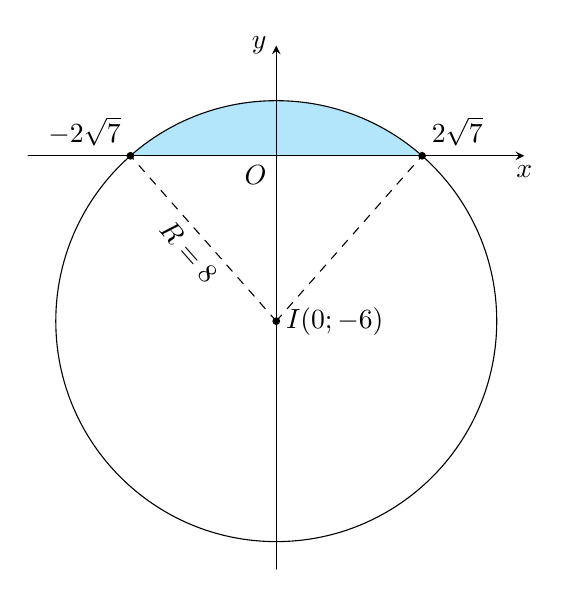
\begin{tikzpicture}[line join=round, line cap=round, >=stealth, scale=0.35]
				\begin{scope}
					\clip (-6,0) rectangle (6,3);
					\fill[cyan!30] (0,-6) circle (8);
				\end{scope}
				\draw[->] (-9,0) -- (9,0) node[below] {$x$};
				\draw[->] (0,-15) -- (0,4) node[left] {$y$};
				\node[below left] at (0,0) {$O$};
				\draw (0,-6) circle (8);
				\fill (0,-6) circle (4pt) node[right] {$I(0;-6)$};
				\draw[dashed] (0,-6) -- ({-sqrt(28)},0) node[sloped,pos=0.5,below] {$R=8$};
				\draw[dashed] (0,-6) -- ({sqrt(28)},0);
				\fill ({-sqrt(28)},0) circle (4pt) node[above left] {$-2\sqrt{7}$};
				\fill ({sqrt(28)},0) circle (4pt) node[above right] {$2\sqrt{7}$};
			\end{tikzpicture}
		\end{center}
		\begin{itemchoice}
			\itemch Từ phương trình đường tròn $(C)\colon x^2+(y+6)^2=8^2$, ta suy ra $(C)$ có tâm $I(0;-6)$ và bán kính $R=\sqrt{8^2}=8$.
			\itemch Phương trình hoành độ giao điểm của $(C)$ và trục hoành $Ox$ (có phương trình $y=0$) là
			\allowdisplaybreaks
			\begin{eqnarray*}
				&&x^2+(0+6)^2=64\\
				&\Leftrightarrow& x^2+36=64 \\
				&\Leftrightarrow& x^2=28 \\
				&\Leftrightarrow& x=\pm 2\sqrt{7}.
			\end{eqnarray*}
			Độ dài dây cung tạo bởi $(C)$ và trục $Ox$ là $2\sqrt{7}-\left(-2\sqrt{7}\right)=4\sqrt{7}$.
			\itemch Từ phương trình của $(C)$ ta suy ra $y+6=\pm\sqrt{64-x^2}$.
			\\
			Do phần hình phẳng $(H)$ nằm phía trên trục hoành nên ta lấy phần đường tròn phía trên có phương trình $y=-6+\sqrt{64-x^2}$ với điều kiện $-6+\sqrt{64-x^2}\ge 0\Leftrightarrow x\in\left[-2\sqrt{7};2\sqrt{7}\right]$.\\
			Diện tích của hình phẳng $(H)$ là
			\[S=\displaystyle\int\limits_{-2\sqrt{7}}^{2\sqrt{7}}\left(-6+\sqrt{64-x^2}\right)\mathrm{\,d}x\approx 14{,}5.\]
			
			\itemch Thể tích khối tròn xoay thu được khi cho $(H)$ quay quanh trục hoành là
			\[V=\pi\displaystyle\int\limits_{-2\sqrt{7}}^{2\sqrt{7}}\left(-6+\sqrt{64-x^2}\right)^2\mathrm{\,d}x=\pi\displaystyle\int\limits_{-2\sqrt{7}}^{2\sqrt{7}}\left(100-x^2-12\sqrt{64-x^2}\right)\mathrm{\,d}x\approx 73{,}8.\]
		\end{itemchoice}
	}
\end{ex}
\caukq
\begin{ex}%[2H5V3-4]%[TDMZZ23]%[Lê Hồ Quang Minh]
	Trong không gian $Oxyz$ có đơn vị dài trên mỗi trục là $400$ kilômét, bề mặt Trái Đất là mặt cầu có phương trình $x^2 + y^2 + z^2 = 256$ và có một tầng điện li coi như là mặt cầu có phương trình $x^2 + y^2 + z^2 = 289$. Từ một điểm $A$ trên mặt đất có một sóng điện từ truyền thẳng, tạo với phương ngang tại $A$ một góc $60^\circ$ (phương ngang tại $A$ là phương tiếp tuyến với Trái Đất tại $A$ và tiếp tuyến này nằm trong mặt phẳng chứa phương truyền của sóng điện từ và tâm của Trái Đất), sóng điện từ này gặp tầng điện li tại điểm $B$. Hãy tính theo đơn vị kilômét độ dài đoạn $A B$ \textit{(không làm tròn ở các phép tính trung gian và làm tròn kết quả cuối cùng đến hàng đơn vị)}?
	\par\shortans[oly]{457}
	\loigiai{
		\immini{
			Xét mặt phẳng cắt đi qua tâm $O$ của Trái Đất, điểm $A$ và điểm $B$.\\
			Thiết diện thu được gồm hai đường tròn đồng tâm $O$
			\begin{itemize}
				\item Đường tròn Trái Đất có bán kính theo đơn vị trục
				\[R_1 = \sqrt{256} = 16.\]
				\item Đường tròn tầng điện li có bán kính theo đơn vị trục
				\[R_2 = \sqrt{289} = 17.\]
			\end{itemize}
			Gọi $At$ là tia tiếp tuyến với đường tròn Trái Đất tại $A$ (phương ngang) $\Rightarrow OA \perp At$ tại $A$.\\
			Theo giả thiết, phương truyền sóng $AB$ tạo với tiếp tuyến $At$ một góc $60^\circ \Rightarrow \widehat{tAB} = 60^\circ$.\\
			Suy ra
			$\widehat{OAB} = \widehat{OAt} + \widehat{tAB} = 90^\circ + 60^\circ = 150^\circ.$
		}{
			\begin{tikzpicture}[scale=0.9, font=\footnotesize, line join=round, line cap=round, >=stealth]
				% 1. Định tâm O và định nghĩa bán kính trực quan cho 2 đường tròn
				\coordinate (O) at (0,0);
				\def\Rone{2.2} % Bán kính Trái Đất (đường tròn trong)
				\def\Rtwo{3.5} % Bán kính Tầng điện li (đường tròn ngoài)
				
				% 2. Vẽ hai đường tròn đồng tâm
				\draw[line width=0.8pt, blue!70] (O) circle (\Rone cm); 
				\draw[line width=0.6pt, dashed, red!70] (O) circle (\Rtwo cm); 
				
				% 3. Định vị điểm A trên bề mặt Trái Đất (góc 110 độ để hình hướng lên đẹp)
				\coordinate (A) at (110:\Rone);
				
				% 4. Dựng tia tiếp tuyến At (phương ngang) vuông góc với OA tại A
				% Góc OA là 110 độ nên góc của tiếp tuyến At sẽ là 110 - 90 = 20 độ
				\coordinate (t) at ($(A)+(20:2.5)$); 
				
				% 5. Dựng tia phát sóng từ A tạo với At góc 60 độ (tức là góc hướng 20 + 60 = 80 độ)
				% Định nghĩa một điểm phụ 'S' nằm xa trên hướng phát sóng
				\coordinate (S) at ($(A)+(80:4)$);
				
				% 6. Tự động tìm giao điểm B của tia phát sóng AS và đường tròn tầng điện li (red)
				% Sử dụng thư viện \usetikzlibrary{intersections}
				\path[name path=lineAB] (A)--(S);
				\path[name path=circleLi] (O) circle (\Rtwo cm);
				\path[name intersections={of=lineAB and circleLi, by=B}];
				
				% 7. Vẽ các đoạn thẳng liên kết thực tế sau khi đã tìm được điểm B chuẩn
				\draw[line width=0.8pt] (O)--(A) node[midway, left] {$R_1$};
				\draw[line width=0.8pt] (O)--(B) node[midway, right, xshift=2pt] {$R_2$};
				\draw[line width=1.1pt, ->, green!60!black] (A)--(B) node[midway, left, xshift=-1pt] {Sóng};
				\draw[line width=0.7pt, black!60] (A)--(t) node[right] {$t$};
				
				% 8. Ký hiệu các góc phẳng
				\pic[draw, angle eccentricity=1, angle radius=2mm]{right angle=O--A--t};
				\pic[draw, angle eccentricity=1.5, angle radius=4mm, "60$^\circ$"] {angle = t--A--B};
				
				% 9. Chấm điểm nút và dán nhãn
				\fill[black] (O) circle (1.2pt) node[below] {$O$};
				\fill[black] (A) circle (1pt) node[left, yshift=-2pt] {$A$};
				\fill[black] (B) circle (1pt) node[above] {$B$};
				
				% Ghi chú tên các thành phần
				\node[blue, font=\tiny] at (-20:\Rone+0.2) {Trái Đất};
				\node[red, font=\tiny] at (-20:\Rtwo+0.2) {Điện li};
			\end{tikzpicture}
		}
		\noindent Áp dụng định lý cosin trong tam giác $OAB$ ta có
		\allowdisplaybreaks
		\begin{eqnarray*}
			&& OB^2 = OA^2 + AB^2 - 2 \cdot OA \cdot AB \cdot \cos\widehat{OAB} \\
			&\Leftrightarrow& 17^2 = 16^2 + AB^2 - 2 \cdot 16 \cdot AB \cdot \cos 150^\circ \\
			&\Leftrightarrow& 289 = 256 + AB^2 - 32AB \cdot \left(-\dfrac{\sqrt{3}}{2}\right) \\
			&\Leftrightarrow& AB^2 + 16\sqrt{3}AB - 33 = 0\\
			&\Leftrightarrow& \hoac{&AB = 15-8\sqrt{3}\\&AB = -15 - 8\sqrt{3}.}
		\end{eqnarray*}
		Vì $AB > 0$ nên $AB = 15 -8\sqrt{3}$.\\
		Vậy độ dài đoạn $AB$ thực tế là $\left(15-8\sqrt{3}\right)\cdot 400 \approx 457$ (km).
	}
\end{ex}
\begin{ex}%[Dự án]%[Tên file]%[1D5V1-3]
	Cho một mẫu số liệu ghép nhóm $M$ với bảng tần số ghép nhóm như sau:
	\begin{center}
		\begin{tabular}{c|c|c|c|c|c|c}
			Nhóm & $[2;3)$ & $[3;4)$ & $[4;5)$ & $[5;6)$ & $[6;7)$ & $[7;8)$ \\
			\hline
			Tần số & $5$ & $4$ & $6$ & $m$ & $8$ & $4$
		\end{tabular}
	\end{center}
	Biết số trung bình cộng của mẫu số liệu sau khi tính toán và được làm tròn đến hàng phần mười là $5{,}2$. Hỏi có tất cả bao nhiêu giá trị của tần số $m$ thoả mãn bài toán?
	\shortans[]{14}
	\loigiai{
		Giá trị đại diện của các nhóm lần lượt là: $c_1=2{,}5$; $c_2=3{,}5$; $c_3=4{,}5$; $c_4=5{,}5$; $c_5=6{,}5$; $c_6=7{,}5$.
		Cỡ mẫu là $n=5+4+6+m+8+4=27+m$ (điều kiện $m \in \mathbb{N}$).
		Số trung bình cộng của mẫu số liệu là
		\[ \overline{x}=\dfrac{2{,}5 \cdot 5+3{,}5 \cdot 4+4{,}5 \cdot 6+5{,}5 \cdot m+6{,}5 \cdot 8+7{,}5 \cdot 4}{27+m}=\dfrac{135{,}5+5{,}5m}{27+m}. \]
		Theo giả thiết, số trung bình cộng làm tròn đến hàng phần mười là $5{,}2$ nên giá trị thực tế của nó nằm trong nửa khoảng $[5{,}15; 5{,}25)$. Ta có hệ bất phương trình:
		\begin{eqnarray*}
			5{,}15 \le \dfrac{135{,}5+5{,}5m}{27+m} < 5{,}25 &\Leftrightarrow& \heva{&135{,}5+5{,}5m \ge 5{,}15(27+m)\\&135{,}5+5{,}5m < 5{,}25(27+m)} \\
			&\Leftrightarrow& \heva{&135{,}5+5{,}5m \ge 139{,}05+5{,}15m\\&135{,}5+5{,}5m < 141{,}75+5{,}25m} \\
			&\Leftrightarrow& \heva{&0{,}35m \ge 3{,}55\\&0{,}25m < 6{,}25} \\
			&\Leftrightarrow& \heva{&m \ge \dfrac{71}{7} \approx 10{,}14\\&m < 25.}
		\end{eqnarray*}
		Vì $m \in \mathbb{N}$ nên $m \in \{11;12;\ldots;24\}$.
		Số các giá trị của $m$ thỏa mãn là $24-11+1=14$.
		Vậy có tất cả $14$ giá trị của tần số $m$ thỏa mãn bài toán.
	}
\end{ex}

\begin{ex}%[2H2C2-5]%[TDMZZ23-19-TLN]
	Cho hình chóp $S. ABCD$ có đáy là hình bình hành với $AB=4$, $AD=6$, $\widehat{ABC}=120^\circ$, có cạnh bên $SA$ vuông góc với đáy $(ABCD)$ và số đo góc nhị diện $[B, SC, D]$ bằng $45^\circ$. Hãy tính thể tích khối chóp $S. ABCD$ (không làm tròn ở các phép tính trung gian và làm tròn kết quả cuối cùng đến hàng đơn vị).
	\par\shortans{14}
	\loigiai{
		\immini{
			Dựng hệ trục tọa độ $Oxyz$ như hình vẽ, sao cho $Oy\perp AB$. Gọi $H$, $K$ lần lượt là hình chiếu vuông góc của $D$ lên các trục $Ox$, $Oy$.\\
			Ta có $AF=DH=AD\cdot \sin \widehat{DAH}=6\cdot \sin 60^\circ=3\sqrt{3}$.\\
			$AH=AD\cdot \cos \widehat{DAH}=6\cdot \cos 60^\circ=3$.\\
			Gọi $E$ là hình chiếu của $C$ lên $Ox$, ta có $AE=AB+BE=7$.\\
			Đặt $SA=h$, khi đó $B(4;0;0)$, $C(7;3\sqrt{3};0)$, $D(3;3\sqrt{3};0)$, $S(0;0;h)$.\\
			Khi đó $\overrightarrow{SC}=(7;3\sqrt{3};-h)$; $\overrightarrow{SB}=(4;0;-h)$; $\overrightarrow{SD}=(3;3\sqrt{3};-h)$.\\
			Véc-tơ pháp tuyến của mặt $(SCB)$ là
			$$\overrightarrow{n}_{(SCB)}=\left[\overrightarrow{SC}, \overrightarrow{SB}\right]=-3\left(h\sqrt{3};-h;4\sqrt{3}\right)\Rightarrow \overrightarrow{n}_1=\left(h\sqrt{3};-h;4\sqrt{3}\right).$$
			Véc-tơ pháp tuyến của mặt $(SCD)$ là
			$$\overrightarrow{n}_{(SCD)}=\left[\overrightarrow{SC}, \overrightarrow{SD}\right]=4\left(0;h;3\sqrt{3}\right)\Rightarrow \overrightarrow{n}_2=\left(0;h;3\sqrt{3}\right).$$
		}
		{\begin{tikzpicture}[line join = round, line cap = round,>=stealth,font=\footnotesize,scale=0.8]
				\def\a{4}   \def\b{3}  \def\h{5}
				\path 
				(0:0) coordinate(A)
				(0:\b) coordinate(D)
				(-40:\a) coordinate(B)
				(90:\h) coordinate(S)
				($(B)+(D)-(A)$) coordinate(C)
				($(A)!1.3!(B)$) coordinate(E)
				($(A)+(C)-(E)$) coordinate(F)
				($(A)+(D)-(F)$) coordinate(H)
				(intersection of A--F and S--C) coordinate(K);
				\draw (A)--(B)--(C) (S)--(A) (S)--(B) (S)--(C)
				(B)--(E)--(C);
				\draw[dashed] (A)--(D)--(C) (S)--(D) (A)--(F)--(D) (F)--(K) (D)--(H);
				\draw pic[draw,angle radius=2mm]{right angle=A--F--D};
				\draw pic[draw,angle radius=2mm]{right angle=C--E--A};
				\draw pic[draw,angle radius=2mm]{right angle=D--H--A};
				\draw[->] (S)--($(A)!1.2!(S)$) node[left]{$z$};
				\draw[->] (B)--($(B)!1.6!(E)$) node[below]{$x$};
				\draw[->] (K)--($(A)!1.2!(K)$) node[below]{$y$};
				\foreach \d/\g in{A/180,B/-150,C/0,D/0,S/0,H/-90,F/90,E/-90}
				\draw[fill=black](\d)circle(1pt)node[shift={(\g:0.25)}]{$\d$};
		\end{tikzpicture}}
		\noindent
		Do đó
		$$\cos[B, SC, D]=\dfrac{\overrightarrow{n}_1\cdot\overrightarrow{n}_2}{\left|\overrightarrow{n}_1\right| \cdot\left| \overrightarrow{n}_2 \right|}=\dfrac{-h^2+36}{\sqrt{4h^2+48}\cdot \sqrt{h^2+27}}=\cos 45^\circ\Rightarrow h\approx 2{,}0499.$$
		Từ đó ta có
		$$V_{S. ABCD}=\dfrac{1}{3}\cdot S_{ABCD}\cdot SA=\dfrac{1}{3}\cdot AB\cdot AD\sin \widehat{BAD}\cdot SA\approx\dfrac{1}{3}\cdot 4\cdot 6\cdot \sin 60^\circ\cdot 2{,}0499\approx 14.$$
	}
\end{ex}

\begin{ex}%[2D4V3-1]%[TDMZZ23]%[Nguyễn Đức Tuấn Anh]
	\immini[thm]{
		Một tam giác đều $ABC$ với độ dài cạnh $AB = 60\text{ cm}$. Hai đường parabol bằng nhau có trục đối xứng lần lượt song song với là $BA$ và $CA$, cắt nhau tại $D$. Biết $BC$ là tiếp tuyến chung của hai parabol và $AD = 14\text{ cm}$. Hãy tính diện tích phần được tô màu theo đơn vị centimet vuông (\textit{làm tròn kết quả đến hàng đơn vị})?}{
		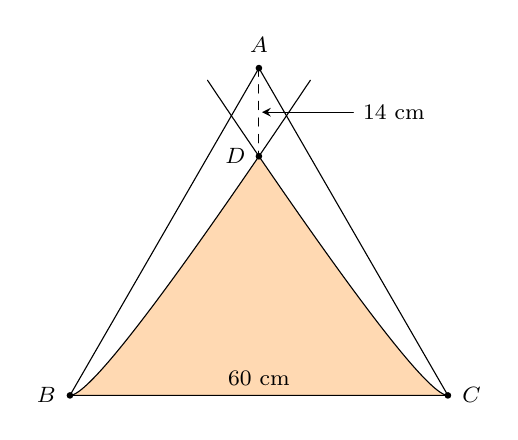
\begin{tikzpicture}[scale=.8, font=\footnotesize, line join=round, line cap=round, >=stealth]
			\pgfmathsetmacro{\h}{3*sqrt(3)}
			\pgfmathsetmacro{\yD}{\h - 1.4}
			\coordinate (A) at (0, \h);
			\coordinate (B) at (-3, 0);
			\coordinate (C) at (3, 0);
			\coordinate (D) at (0, \yD);
			\pgfmathsetmacro{\xCA}{-3 + 1.4*sqrt(3)/9}
			\pgfmathsetmacro{\yCA}{0}
			\pgfmathsetmacro{\xCB}{-2 + 1.4*sqrt(3)/9}
			\pgfmathsetmacro{\yCB}{sqrt(3) - 1.4/3}
			\fill[orange!30] (B) .. controls (\xCA,\yCA) and (\xCB,\yCB) .. (D) .. controls (-\xCB,\yCB) and (-\xCA,\yCA) .. (C) -- cycle;
			\pgfmathsetmacro{\tD}{1.4/sqrt(3)}
			\pgfmathsetmacro{\cD}{(3 - \tD)/(\tD*\tD)}
			\pgfmathsetmacro{\tMax}{\tD + 0.12}
			\draw[] plot[domain=0:\tMax, samples=50] ({-3 + \x + \cD*(\x)^2}, {\cD*sqrt(3)*(\x)^2});
			\draw[] plot[domain=0:\tMax, samples=50] ({3 - \x - \cD*(\x)^2}, {\cD*sqrt(3)*(\x)^2});
			\draw[] (A) -- (B) -- (C) -- cycle;
			\draw[dashed, thin] (A) -- (D);
			\foreach \p/\ang in {A/90, B/180, C/0, D/180}
			\fill (\p) circle (1.5pt)node[shift=(\ang:0.3)]{$\p$};
			\node[above] at (0, 0) {$60$ cm};
			\node[right] at (1.5, {\h - 0.7}) {$14$ cm};
			\draw[->] (1.5, {\h - 0.7}) -- (0.05, {\h - 0.7});
		\end{tikzpicture}
	}
	\par\shortans[]{1\,036}
	\loigiai{
		Chọn hệ trục tọa độ $Oxy$ như hình vẽ.
		\begin{center}
			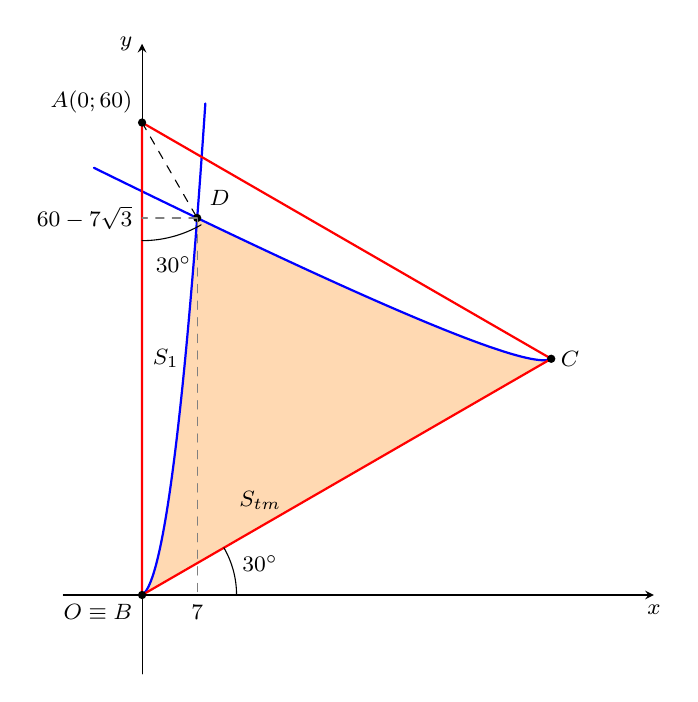
\begin{tikzpicture}[scale=1, font=\footnotesize, line join=round, line cap=round, >=stealth]
				\draw[->] (-1, 0) -- (6.5, 0) node[below] {$x$};
				\draw[->] (0, -1) -- (0, 7) node[left] {$y$};
				\coordinate (O) at (0,0);
				\coordinate (B) at (0,0);
				\coordinate (A) at (0,6);
				\coordinate (C) at ({3*sqrt(3)}, 3);
				\coordinate (D) at (0.7, {6 - 0.7*sqrt(3)});
				\begin{scope}[shift={({1.5*sqrt(3)}, 1.5)}, rotate=30]
					\pgfmathsetmacro{\h}{3*sqrt(3)}
					\pgfmathsetmacro{\yD}{\h - 1.4}
					\pgfmathsetmacro{\xCA}{-3 + 1.4*sqrt(3)/9}
					\pgfmathsetmacro{\yCA}{0}
					\pgfmathsetmacro{\xCB}{-2 + 1.4*sqrt(3)/9}
					\pgfmathsetmacro{\yCB}{sqrt(3) - 1.4/3}
					\fill[orange!30] (-3,0) .. controls (\xCA,\yCA) and (\xCB,\yCB) .. (0,\yD) .. controls (-\xCB,\yCB) and (-\xCA,\yCA) .. (3,0) -- cycle;
					
					\pgfmathsetmacro{\tD}{1.4/sqrt(3)}
					\pgfmathsetmacro{\cD}{(3 - \tD)/(\tD*\tD)}
					\pgfmathsetmacro{\tMax}{\tD + 0.12}
					\draw[blue, thick] plot[domain=0:\tMax, samples=50] ({-3 + \x + \cD*(\x)^2}, {\cD*sqrt(3)*(\x)^2});
					\draw[blue, thick] plot[domain=0:\tMax, samples=50] ({3 - \x - \cD*(\x)^2}, {\cD*sqrt(3)*(\x)^2});
				\end{scope}
				
				\draw[red, thick] (A) -- (B) -- (C) -- cycle;
				\draw[dashed, thin] (A) -- (D);
				
				\fill (O) circle (1.5pt) node[below left] {$O \equiv B$};
				\fill (A) circle (1.5pt) node[above left] {$A(0; 60)$};
				\fill (C) circle (1.5pt) node[right] {$C$};
				\fill (D) circle (1.5pt) node[above right=1pt] {$D$};
				
				\draw[dashed, thin, gray] (D) -- (0.7, 0) node[below, text=black] {$7$};
				\draw[dashed, thin, gray] (D) -- (0, {6 - 0.7*sqrt(3)}) node[left, text=black] {$60-7\sqrt{3}$};
				
				\draw (1.2, 0) arc (0:30:1.2);
				\node at (1.5, 0.4) {$30^\circ$};
				
				\draw (0, 4.5) arc (-90:-60:1.5);
				\node at (0.4, 4.2) {$30^\circ$};
				\node at (0.3, 3) {$S_1$};
				\node at (1.5, 1.2) {$S_{tm}$};
			\end{tikzpicture}
		\end{center}
		Khi đó, ta có $A(0; 60)$.\\
		Vì tam giác $ABC$ đều nên $\widehat{ABC} = 60^\circ$. Đường thẳng $BC$ tạo với trục $Oy$ góc $60^\circ$, suy ra tạo với trục $Ox$ góc $30^\circ$. \\
		Đường thẳng $BC$ đi qua gốc tọa độ $O$ và có hệ số góc $k = \tan 30^\circ = \dfrac{1}{\sqrt{3}}$ nên có phương trình: $y = \dfrac{1}{\sqrt{3}}x$.\\
		Đường cao từ $A$ cũng là đường phân giác góc $\widehat{A}$, do đó đường thẳng $AD$ tạo với trục $Oy$ một góc $30^\circ$.\\
		Vì $AD = 14$ nên toạ độ của điểm $D$ là $\heva{x_D &= 14 \sin 30^\circ = 7\\y_D &= 60 - 14 \cos 30^\circ = 60 - 7\sqrt{3}.}$\\
		Vậy $D\left(7; 60 - 7\sqrt{3}\right)$.\\
		Đường parabol bên trái (kí hiệu là $(P)$) có trục đối xứng song song với $BA$ (trục $Oy$) nên phương trình có dạng $y = f(x) = ax^2 + bx + c$.\\
		Parabol $(P)$ tiếp xúc với $BC$ tại $B(0;0)$ nên đi qua gốc tọa độ $O \Rightarrow c = 0$, đồng thời $f'(0)$ bằng hệ số góc của $BC$ nên
		\[ f'(0) = b = \dfrac{1}{\sqrt{3}}. \]
		Mà parabol $(P)$ đi qua điểm $D$ nên
		\[ a \cdot 7^2 + 7 \cdot \dfrac{1}{\sqrt{3}} = 60 - 7\sqrt{3} \Rightarrow a = \dfrac{1}{49}\left(60 - \dfrac{28\sqrt{3}}{3}\right). \]
		Vậy $(P)\colon \dfrac{1}{49}\left(60 - \dfrac{28\sqrt{3}}{3}\right)x^2+ \dfrac{1}{\sqrt{3}}x$.\\
		Gọi $S_1$ là diện tích phần không tô màu bên trái. \\
		Đường thẳng $AD$ đi qua $A(0; 60)$ và $D\left(7; 60 - 7\sqrt{3}\right)$ có hệ số góc $k_{AD} = \dfrac{60 - 7\sqrt{3} - 60}{7 - 0} = -\sqrt{3}$ nên có phương trình $y = -\sqrt{3}x + 60$.\\
		Ta có $S_1$ là diện tích hình phẳng giới hạn bởi trục $Oy$ (cạnh $AB$), đường thẳng $AD$ và parabol $(P)$, do đó
		\[	S_1 = \displaystyle\int\limits_0^7 \left[ \left(-\sqrt{3}x + 60\right) - \left( \dfrac{1}{49}\left(60 - \dfrac{28\sqrt{3}}{3}\right)x^2+ \dfrac{1}{\sqrt{3}}x\right) \right] \mathrm{d}x =280 - \dfrac{98\sqrt{3}}{9}\,\left(\text{cm}^2\right)\]
		Diện tích tam giác đều $ABC$ là $S_{\triangle ABC} = \dfrac{\sqrt{3}}{4} \cdot 60^2 = 900\sqrt{3}\,\left(\text{cm}^2\right)$.\\
		Diện tích phần được tô màu là
		\[S = S_{\triangle ABC} - 2S_1 = 900\sqrt{3} - 2\left( 280 - \dfrac{98\sqrt{3}}{9} \right) \approx 1\,036\,\left(\text{cm}^2\right).\]
	}
\end{ex}
\begin{ex}%[Dự án]%[Tên file]%[1D9C2-4]
	Theo thống kê hiện tại có một dịch bệnh X rất nguy hiểm và đang có $4\%$ dân số thật sự mắc bệnh này. Một công ty có đề xuất một loại dụng cụ TEST X cho khả năng phát hiện chuẩn đến $90\%$ một loại bệnh X (tức là một người bị bệnh X khi dùng dụng cụ TEST X sẽ cho xác suất dương tính là $90\%$). Tuy nhiên, TEST X cũng cho kết quả ``dương tính giả'' cho một người không bị bệnh X tới $5\%$ (tức là một người không bị bệnh X mà dùng TEST X sẽ cho kết quả dương tính là $5\%$). Một người dùng TEST X này $4$ lần liên tiếp, kết quả các lần TEST là độc lập với nhau. Gọi $p$ là xác suất để người này thật sự bị bệnh X, nếu nhận được kết quả dương tính đúng $3$ lần. Hãy tính $10000p$ (làm tròn kết quả đến hàng đơn vị)?
	\shortans[]{9624}
	\loigiai{
		Gọi $A$ là biến cố ``Người đó thật sự mắc bệnh X''. Ta có $\mathrm{P}(A) = 0{,}04 \Rightarrow \mathrm{P}(\overline{A}) = 0{,}96$.
		Gọi $B$ là biến cố ``Một lần TEST cho kết quả dương tính''.
		Theo giả thiết, ta có:
		\begin{itemize}
			\item Xác suất TEST dương tính khi người đó có bệnh là $\mathrm{P}(B|A) = 0{,}9$.
			\item Xác suất TEST âm tính khi người đó có bệnh là $\mathrm{P}(\overline{B}|A) = 1 - 0{,}9 = 0{,}1$.
			\item Xác suất TEST dương tính khi người đó không có bệnh là $\mathrm{P}(B|\overline{A}) = 0{,}05$.
			\item Xác suất TEST âm tính khi người đó không có bệnh là $\mathrm{P}(\overline{B}|\overline{A}) = 1 - 0{,}05 = 0{,}95$.
		\end{itemize}
		Gọi $B_4^3$ là biến cố ``Nhận được kết quả dương tính đúng $3$ lần trong $4$ lần TEST''.
		Xác suất để có đúng $3$ lần TEST dương tính trong $4$ lần thử khi biết người đó mắc bệnh là
		\[ \mathrm{P}(B_4^3|A) = \mathrm{C}_4^3 \cdot [\mathrm{P}(B|A)]^3 \cdot [\mathrm{P}(\overline{B}|A)]^1 = 4 \cdot 0{,}9^3 \cdot 0{,}1 = 0{,}2916. \]
		Xác suất để có đúng $3$ lần TEST dương tính trong $4$ lần thử khi biết người đó không mắc bệnh là
		\[ \mathrm{P}(B_4^3|\overline{A}) = \mathrm{C}_4^3 \cdot [\mathrm{P}(B|\overline{A})]^3 \cdot [\mathrm{P}(\overline{B}|\overline{A})]^1 = 4 \cdot 0{,}05^3 \cdot 0{,}95 = 0{,}000475. \]
		Theo công thức Bayes, xác suất người đó thật sự mắc bệnh khi có $3$ lần TEST dương tính là
		\begin{eqnarray*}
			p = \mathrm{P}(A|B_4^3) &=& \dfrac{\mathrm{P}(B_4^3|A) \cdot \mathrm{P}(A)}{\mathrm{P}(B_4^3|A) \cdot \mathrm{P}(A) + \mathrm{P}(B_4^3|\overline{A}) \cdot \mathrm{P}(\overline{A})} \\
			&=& \dfrac{0{,}2916 \cdot 0{,}04}{0{,}2916 \cdot 0{,}04 + 0{,}000475 \cdot 0{,}96} \\
			&\approx& 0{,}96237.
		\end{eqnarray*}
		Suy ra $10000p \approx 9623{,}7$. Làm tròn đến hàng đơn vị ta được $9624$.
	}
\end{ex}
\begin{ex}%[0D8C2-7]%[TDM42]
	Có $14$ chiếc ghế chia thành hai hàng ngang và thành $7$ cặp đối diện nhau, mỗi chiếc ghế chỉ ngồi được một người. Gọi $T$ là số cách xếp $4$ em lớp $A$, $3$ em lớp $B$, $2$ em học sinh lớp $C$, $1$ học sinh lớp $D$, $1$ học sinh lớp $E$ vào $14$ ghế này sao cho không có học sinh nào cùng lớp ngồi đối diện nhau. Hãy tính $\dfrac{T}{10^6}$ \textit{(làm tròn kết quả đến hàng đơn vị)}?
	\begin{center}
		\begin{tikzpicture}[scale=0.9, >=stealth]
			% Vẽ 7 cặp ghế đối diện nhau (Hàng 1 và Hàng 2)
			\foreach \x in {1,...,7} {
				% Ghế hàng 1 (màu xanh nhẹ)
				\draw[thick, fill=cyan!8, draw=cyan!60!black, rounded corners=3pt] (\x*1.4-0.5, 0.7) rectangle ++(1.0,1.0);
				\node[cyan!80!black, font=\small\bfseries] at (\x*1.4, 1.2) {\x};
				
				% Ghế hàng 2 (màu cam nhẹ)
				\draw[thick, fill=orange!8, draw=orange!60!black, rounded corners=3pt] (\x*1.4-0.5, -1.1) rectangle ++(1.0,1.0);
				\node[orange!80!black, font=\small\bfseries] at (\x*1.4, -0.6) {\x$'$};
				
				% Mũi tên biểu diễn quan hệ đối diện
				\draw[<->, dashed, gray!80, thick] (\x*1.4, 0.5) -- (\x*1.4, -0.2);
			}
			
			% Nhãn chỉ hướng hàng ghế
			\node[anchor=east, cyan!60!black, font=\bfseries\small] at (0.6, 1.2) {Hàng 1 $\rightarrow$};
			\node[anchor=east, orange!60!black, font=\bfseries\small] at (0.6, -0.6) {Hàng 2 $\rightarrow$};
			
			% Chú thích cặp đối diện
			\node[anchor=west, gray!70!black, font=\itshape\small] at (11.0, 0.3) {* Các cặp đối diện:};
			\node[anchor=west, gray!70!black, font=\itshape\small] at (11.0, -0.3) {$(1,1'), (2,2'), \dots, (7,7')$};
		\end{tikzpicture}
	\end{center}
	\par\shortans[0]{6077}
	\loigiai{
		\textbf{Cách 1: (Dùng Phương pháp Trực tiếp và Nguyên lí bù trừ)}\\
		\textbf{Bước 1: Tính số cách sắp xếp tổng quát (không ràng buộc)}\\
		Tổng số học sinh tham gia sắp xếp là: $4 + 3 + 2 + 1 + 1 = 11$ học sinh.
		Xếp ngẫu nhiên $11$ học sinh phân biệt vào $14$ chiếc ghế phân biệt, số cách sắp xếp ngẫu nhiên là chỉnh hợp chập $11$ của $14$
		$$N = \mathrm{A}_{14}^{11} = \dfrac{14!}{3!} = 14.529.715.200 \text{ (cách)}$$
		\textbf{Bước 2: Phân tích các trường hợp vi phạm bằng Nguyên lí bù trừ}
		Một cách xếp vị trí bị coi là \textit{vi phạm} nếu tồn tại ít nhất một cặp ghế đối diện nhau chứa hai học sinh thuộc cùng một lớp.
		Vì các lớp $D$ và $E$ chỉ có duy nhất $1$ học sinh nên hiện tượng vi phạm đối diện cùng lớp chỉ có thể xảy ra ở các lớp $A$ (có 4 em), lớp $B$ (có 3 em), hoặc lớp $C$ (có 2 em).
		\\Gọi
		\begin{itemize}
			\item $k_A$ là số cặp ghế đối diện chứa hai học sinh lớp $A$ ($0 \le k_A \le 2$).
			\item $k_B$ là số cặp ghế đối diện chứa hai học sinh lớp $B$ ($0 \le k_B \le 1$).
			\item $k_C$ là số cặp ghế đối diện chứa hai học sinh lớp $C$ ($0 \le k_C \le 1$).
		\end{itemize}
		Với mỗi bộ số $(k_A, k_B, k_C)$ xác định, số cách chọn ghế và sắp xếp các học sinh vi phạm kết hợp xếp các học sinh còn lại được thực hiện theo quy trình sau:
		\begin{enumerate}
			\item \textbf{Chọn các cặp ghế vi phạm:} Chọn $k_A$ cặp từ 7 cặp ghế ban đầu, chọn tiếp $k_B$ cặp từ $7-k_A$ cặp còn lại, và chọn $k_C$ cặp từ $7-k_A-k_B$ cặp còn lại. Số cách chọn cặp ghế là: $\mathrm{C}_7^{k_A} \cdot \mathrm{C}_{7-k_A}^{k_B} \cdot \mathrm{C}_{7-k_A-k_B}^{k_C}$.
			\item \textbf{Xếp học sinh vào các cặp vi phạm đã chọn:}
			\begin{itemize}
				\item Chọn và xếp học sinh lớp $A$ vào $k_A$ cặp ghế: $\mathrm{A}_4^{2k_A}$ cách.
				\item Chọn và xếp học sinh lớp $B$ vào $k_B$ cặp ghế: $\mathrm{A}_3^{2k_B}$ cách.
				\item Chọn và xếp học sinh lớp $C$ vào $k_C$ cặp ghế: $\mathrm{A}_2^{2k_C}$ cách.
			\end{itemize}
			\item \textbf{Xếp các học sinh còn lại vào các ghế trống tự do:}
			Sau khi xếp xong các cặp vi phạm, số ghế còn dư lại là $14 - 2(k_A+k_B+k_C)$ và số học sinh còn lại cần xếp là $11 - 2(k_A+k_B+k_C)$. Số cách xếp phần còn lại là: $\mathrm{A}_{14 - 2(k_A+k_B+k_C)}^{11 - 2(k_A+k_B+k_C)}$.
		\end{enumerate}
		\textbf{Bước 3: Lập bảng tính chi tiết các thành phần bù trừ}\\
		Theo Nguyên lí bù trừ, số cách sắp xếp thỏa mãn yêu cầu không đối diện cùng lớp là:
		$$T = \sum_{k_A, k_B, k_C} (-1)^{k_A + k_B + k_C} \cdot \left[ \text{Số cách xếp ứng với bộ } (k_A, k_B, k_C) \right]$$
		Ta có bảng tổng hợp giá trị của tất cả các bộ thành phần chi tiết như sau
		\begin{center}
			\small
			\renewcommand{\arraystretch}{1.3}
			\begin{tabular}{|c|c|c|c|l|r|}
				\hline
				$\mathbf{k_A}$ & $\mathbf{k_B}$ & $\mathbf{k_C}$ & \textbf{Dấu} & \textbf{Công thức tính số cách xếp thành phần} & \textbf{Giá trị thành phần} \\ \hline
				0 & 0 & 0 & $+$ & $\mathrm{C}_7^0 \cdot \mathrm{C}_7^0 \cdot \mathrm{C}_7^0 \cdot \mathrm{A}_4^0 \cdot \mathrm{A}_3^0 \cdot \mathrm{A}_2^0 \cdot \mathrm{A}_{14}^{11}$ & $14.529.715.200$ \\ \hline
				0 & 0 & 1 & $-$ & $\mathrm{C}_7^0 \cdot \mathrm{C}_7^0 \cdot \mathrm{C}_7^1 \cdot \mathrm{A}_4^0 \cdot \mathrm{A}_3^0 \cdot \mathrm{A}_2^2 \cdot \mathrm{A}_{12}^9$ & $-1.117.670.400$ \\ \hline
				0 & 1 & 0 & $-$ & $\mathrm{C}_7^0 \cdot \mathrm{C}_7^1 \cdot \mathrm{C}_6^0 \cdot \mathrm{A}_4^0 \cdot \mathrm{A}_3^2 \cdot \mathrm{A}_2^0 \cdot \mathrm{A}_{12}^9$ & $-3.353.011.200$ \\ \hline
				0 & 1 & 1 & $+$ & $\mathrm{C}_7^0 \cdot \mathrm{C}_7^1 \cdot \mathrm{C}_6^1 \cdot \mathrm{A}_4^0 \cdot \mathrm{A}_3^2 \cdot \mathrm{A}_2^2 \cdot \mathrm{A}_{10}^7$ & $304.819.200$ \\ \hline
				1 & 0 & 0 & $-$ & $\mathrm{C}_7^1 \cdot \mathrm{C}_6^0 \cdot \mathrm{C}_6^0 \cdot \mathrm{A}_4^2 \cdot \mathrm{A}_3^0 \cdot \mathrm{A}_2^0 \cdot \mathrm{A}_{12}^9$ & $-6.706.022.400$ \\ \hline
				1 & 0 & 1 & $+$ & $\mathrm{C}_7^1 \cdot \mathrm{C}_6^0 \cdot \mathrm{C}_6! \cdot \mathrm{A}_4^2 \cdot \mathrm{A}_3^0 \cdot \mathrm{A}_2^2 \cdot \mathrm{A}_{10}^7$ & $609.638.400$ \\ \hline
				1 & 1 & 0 & $+$ & $\mathrm{C}_7^1 \cdot \mathrm{C}_6^1 \cdot \mathrm{C}_5^0 \cdot \mathrm{A}_4^2 \cdot \mathrm{A}_3^2 \cdot \mathrm{A}_2^0 \cdot \mathrm{A}_{10}^7$ & $1.828.915.200$ \\ \hline
				1 & 1 & 1 & $-$ & $\mathrm{C}_7^1 \cdot \mathrm{C}_6^1 \cdot \mathrm{C}_5^1 \cdot \mathrm{A}_4^2 \cdot \mathrm{A}_3^2 \cdot \mathrm{A}_2^2 \cdot \mathrm{A}_8^5$ & $-203.212.800$ \\ \hline
				2 & 0 & 0 & $+$ & $\mathrm{C}_7^2 \cdot \mathrm{C}_5^0 \cdot \mathrm{C}_5^0 \cdot \mathrm{A}_4^4 \cdot \mathrm{A}_3^0 \cdot \mathrm{A}_2^0 \cdot \mathrm{A}_{10}^7$ & $304.819.200$ \\ \hline
				2 & 0 & 1 & $-$ & $\mathrm{C}_7^2 \cdot \mathrm{C}_5^0 \cdot \mathrm{C}_5^1 \cdot \mathrm{A}_4^4 \cdot \mathrm{A}_3^0 \cdot \mathrm{A}_2^2 \cdot \mathrm{A}_8^5$ & $-33.868.800$ \\ \hline
				2 & 1 & 0 & $-$ & $\mathrm{C}_7^2 \cdot \mathrm{C}_5^1 \cdot \mathrm{C}_4^0 \cdot \mathrm{A}_4^4 \cdot \mathrm{A}_3^2 \cdot \mathrm{A}_2^0 \cdot \mathrm{A}_8^5$ & $-101.606.400$ \\ \hline
				2 & 1 & 1 & $+$ & $\mathrm{C}_7^2 \cdot \mathrm{C}_5^1 \cdot \mathrm{C}_4^1 \cdot \mathrm{A}_4^4 \cdot \mathrm{A}_3^2 \cdot \mathrm{A}_2^2 \cdot \mathrm{A}_6^3$ & $14.515.200$ \\ \hline
				\multicolumn{5}{|r|}{\textbf{Tổng số cách thỏa mãn ($T$):}} & $\mathbf{6.077.030.400}$ \\ \hline
			\end{tabular}
		\end{center}
		\textbf{Bước 4: Kết luận giá trị yêu cầu}\\
		Từ bảng số liệu thu được từ đại lượng tổng $T$, ta có giá trị biểu thức đề bài yêu cầu là:
		$$\dfrac{T}{10^6} = \dfrac{6.077.030.400}{10^6} = 6077.$$
		\textbf{Cách 2: (Dùng phương pháp loại trừ và chia trường hợp)}\\
		\textbf{Bước 1: Tính số không gian mẫu (Xếp tùy ý)}
		
		Tổng số học sinh là: $4 + 3 + 2 + 1 + 1 = 11$ học sinh. Xếp $11$ học sinh vào $14$ chiếc ghế:
		$$N = \mathrm{A}_{14}^{11} = 14.529.715.200 \text{ (cách)}$$
		
		\textbf{Bước 2: Tư duy "Bù trừ gộp nhóm"}
		
		Một cách xếp bị coi là \textbf{vi phạm} nếu có học sinh cùng lớp ngồi đối diện nhau. Hiện tượng này chỉ có thể xảy ra ở nội bộ lớp $A$, lớp $B$, và lớp $C$.
		Thay vì chia lẻ tẻ từng lớp, ta sẽ đếm \textbf{số cách tạo ra $k$ cặp học sinh cùng lớp} (gọi tắt là "cặp vi phạm") trên toàn bộ các học sinh.
		\begin{itemize}
			\item \textbf{Nội bộ lớp A (4 em):}
			\begin{itemize}
				\item Tạo $0$ cặp vi phạm: có $1$ cách.
				\item Tạo $1$ cặp vi phạm (chọn 2 em): có $\mathrm{C}_4^2 = 6$ cách.
				\item Tạo $2$ cặp vi phạm: có $\dfrac{\mathrm{C}_4^2 \cdot \mathrm{C}_2^2}{2!} = 3$ cách.
			\end{itemize}
			$\Rightarrow$ Đại diện bằng đa thức: $P_A = 1 + 6x + 3x^2$
			
			\item \textbf{Nội bộ lớp B (3 em):}
			\begin{itemize}
				\item Tạo $0$ cặp: $1$ cách. Tạo $1$ cặp: $\mathrm{C}_3^2 = 3$ cách.
			\end{itemize}
			$\Rightarrow$ Đại diện bằng đa thức: $P_B = 1 + 3x$
			
			\item \textbf{Nội bộ lớp C (2 em):}
			\begin{itemize}
				\item Tạo $0$ cặp: $1$ cách. Tạo $1$ cặp: $\mathrm{C}_2^2 = 1$ cách.
			\end{itemize}
			$\Rightarrow$ Đại diện bằng đa thức: $P_C = 1 + x$
		\end{itemize}
		
		Nhân phân phối cả 3 nhóm lại để tìm số cách tạo ra $k$ cặp vi phạm cho toàn trường:
		\begin{align*}
			P &= P_A \cdot P_B \cdot P_C = (1 + 6x + 3x^2)(1 + 3x)(1 + x) \\
			&= \mathbf{1} + \mathbf{10}x + \mathbf{30}x^2 + \mathbf{30}x^3 + \mathbf{9}x^4
		\end{align*}
		\textbf{Ý nghĩa:} Đặt $c_k$ là hệ số của $x^k$. Ta có
		$c_0=1, c_1=10, c_2=30, c_3=30, c_4=9$. Số $c_k$ chính là tổng số cách chọn ra đúng $k$ cặp học sinh vi phạm từ các lớp!
		\textbf{Bước 3: Lập công thức tổng quát tính số cách vi phạm}
		Gọi $S_k$ là \textit{số cách xếp sao cho có xuất hiện $k$ cặp ghế vi phạm}. Để tạo ra $S_k$, ta làm $4$ hành động sau:
		\begin{enumerate}
			\item Chọn ra những học sinh để tạo thành $k$ cặp vi phạm: Có $\mathbf{c_k}$ cách (đã tính ở trên).
			\item Chọn $k$ cặp ghế (trong $7$ cặp ghế) và xếp $k$ cặp học sinh đó vào: Có $\mathbf{A_7^k}$ cách.
			\item Tại mỗi cặp ghế đối diện, 2 học sinh có thể đổi chỗ cho nhau: Có $\mathbf{2^k}$ cách.
			\item Lấy $11 - 2k$ học sinh còn lại xếp tùy ý vào $14 - 2k$ chiếc ghế trống: Có $\mathbf{A_{14 - 2k}^{11 - 2k}}$ cách.
		\end{enumerate}
		Nhân tất cả lại, ta được
		$$S_k = c_k \cdot \mathrm{A}_7^k \cdot 2^k \cdot \mathrm{A}_{14-2k}^{11-2k}$$
		\textbf{Bước 4: Bảng tính bù trừ thu gọn}
		Chỉ với 1 công thức trên, ta lập bảng 5 dòng cho Nguyên lí Bù trừ ($T = S_0 - S_1 + S_2 - S_3 + S_4$):
		\begin{center}
			\renewcommand{\arraystretch}{1.5}
			\begin{tabular}{|c|c|p{0.55\linewidth}|r|}
				\hline
				$\mathbf{k}$ & $\mathbf{c_k}$ & \multicolumn{1}{c|}{\textbf{Công thức tính $S_k$}} & \multicolumn{1}{c|}{\textbf{Giá trị $S_k$}} \\ \hline
				0 & $1$ & $S_0 = 1 \cdot \mathrm{A}_7^0 \cdot 2^0 \cdot \mathrm{A}_{14}^{11}$ & $14.529.715.200$ \\ \hline
				1 & $10$ & $S_1 = 10 \cdot \mathrm{A}_7^1 \cdot 2^1 \cdot \mathrm{A}_{12}^9$ & $11.176.704.000$ \\ \hline
				2 & $30$ & $S_2 = 30 \cdot \mathrm{A}_7^2 \cdot 2^2 \cdot \mathrm{A}_{10}^7$ & $3.048.192.000$ \\ \hline
				3 & $30$ & $S_3 = 30 \cdot \mathrm{A}_7^3 \cdot 2^3 \cdot \mathrm{A}_8^5$ & $338.688.000$ \\ \hline
				4 & $9$ & $S_4 = 9 \cdot \mathrm{A}_7^4 \cdot 2^4 \cdot \mathrm{A}_6^3$ & $14.515.200$ \\ \hline
				\multicolumn{3}{|r|}{\textbf{Tổng $T = S_0 - S_1 + S_2 - S_3 + S_4$ =}} & $\mathbf{6.077.030.400}$ \\ \hline
			\end{tabular}
		\end{center}
		\textbf{Bước 5: Kết luận}
		Từ tổng $T$ thu được, giá trị biểu thức đề bài yêu cầu là:
		$$\dfrac{T}{10^6} = \dfrac{6.077.030.400}{10^6} \approx 6077.$$
	}
\end{ex}